\documentclass[11pt,a4paper]{article}

\usepackage[utf8]{inputenc}
\usepackage[T1]{fontenc}
\usepackage{lmodern}
\usepackage[margin=2.4cm]{geometry}
\usepackage{amsmath,amssymb}
\usepackage{graphicx}
\usepackage{booktabs}
\usepackage{array}
\usepackage{longtable}
\usepackage{enumitem}
\usepackage{caption}
\usepackage{float}
\usepackage{microtype}
\usepackage{hyperref}
\usepackage{siunitx}
\usepackage{xcolor}
\usepackage{fancyhdr}
\usepackage{tikz}

\hypersetup{colorlinks=true,linkcolor=black,urlcolor=blue,citecolor=black}
\sisetup{per-mode=symbol,detect-all,exponent-product=\times}

\pagestyle{fancy}
\fancyhf{}
\lhead{Les sylphes -- reviewed solution}
\rhead{TLE exam}
\cfoot{\thepage}

\setlength{\headheight}{14pt}
\setlength{\parindent}{0pt}
\setlength{\parskip}{0.55em}
\renewcommand{\arraystretch}{1.18}

\newenvironment{finalanswer}{%
  \begin{center}\begin{minipage}{0.94\linewidth}\hrule\vspace{0.45em}\textbf{Final answer. }%
}{%
  \vspace{0.45em}\hrule\end{minipage}\end{center}%
}

\newcommand{\E}{\mathbf{E}}
\newcommand{\B}{\mathbf{B}}
\newcommand{\jv}{\mathbf{j}}
\newcommand{\grad}{\operatorname{grad}}
\newcommand{\RT}{R_T}
\newcommand{\gzero}{g_0}
\newcommand{\ISS}{\mathrm{ISS}}
\newcommand{\Otwo}{\ensuremath{\mathrm{O}_2}}
\newcommand{\Ntwo}{\ensuremath{\mathrm{N}_2}}
\newcommand{\eV}{\ensuremath{\mathrm{eV}}}

\title{Concours Commun Mines-Ponts (CCMP) 2023\\[0.25em]
\large Physics I Exam, PC Track\\[0.8em]
\Large Les sylphes\\[0.25em]
\large Reviewed and Corrected Solution}
\author{}
\date{}

\begin{document}
\maketitle

\tableofcontents
\newpage

\section*{Notes on this revision}
\addcontentsline{toc}{section}{Notes on this revision}

Every numerical result of the previous version was recomputed independently and
every figure was re-read. The physics and the algebra were correct throughout;
the changes below are one arithmetic correction, two arguments that were
incomplete, and a number of places where the figures allow a sharper answer than
was given.

\begin{itemize}[nosep]
\item \textbf{Q8, corrected.} $H=RT_0/(Mg_0)=\SI{8.48}{km}$, which is \SI{8}{km}
to one significant figure, not \SI{9}{km}. The previous value came from rounding
twice ($8.48\to8.5\to9$). This does not affect $\xi=\ell/H\simeq6$ or
$\chi\simeq\SI{1.1e3}{km}$.
\item \textbf{Q19, completed.} The previous argument identified the decay
constant of $N(x)$ rather than computing a mean. The free-path probability
density is now derived and $\langle x\rangle$ integrated.
\item \textbf{Q3, quantified.} The colour bars of Figure 4 give 836~LSB
(visible) and 62~LSB (filtered). The visible reading is exactly one conventional
flash and the filtered reading is about twice what that flash should give, so the
argument is a factor $\simeq2$ excess, not a ``much larger'' ratio. The reason the
\SI{761}{nm} band discriminates by altitude is now stated.
\item \textbf{Q1, sharpened.} The tallest peak of the emission spectrum
(\SI{760}{nm}) is infrared and cannot explain a colour; the red appearance comes
from the \SIrange{640}{690}{nm} group being the only significant emission inside
the visible window.
\item \textbf{Q24, disambiguated.} Figure 7 is calibrated for
$\ell_{pm}=\SI{2}{cm}$, not for the \SI{1}{cm} quoted in the statement; the
back-calculation is now shown, together with the $\mathcal{N}\simeq32$ that a
literal \SI{1}{cm} would give.
\item \textbf{Q7, Q9, Q11, Q12, Q13, Q15, Q17, Q22} were correct and have been
strengthened: ground-track versus orbital speed, the size of the $\varepsilon$
expansion error, numerical temperatures at 20 and \SI{50}{km}, oxygen partial
pressures, a self-consistent bound on $v/c$, a proof that $\rho=0$ rather than an
assertion, the ambient-density contrast behind the radar echoes, and the
$v\simeq2c$ reductio for the relativistic electrons.
\item \textbf{Course-question rigour (Q2, Q4, Q5, Q13, Q14, Q23).} Several
answers stated a standard result instead of establishing it. Gauss' theorem is
now actually applied to a spherical surface rather than invoked for its
conclusion; the constancy of the orbital speed is proved from
$\mathbf v\cdot\mathbf g=0$, as the statement's ``after showing that it is
constant'' requires; the magnetic Lorentz term is bounded using
$\B=(k/\omega)\mathbf e_z\times\E$ and $v/v_\varphi$ rather than the
inapplicable $B=E/c$, since the plasma is dispersive; the ion current is
suppressed by an explicit mass ratio; and the doubling convention of Question 23
is stated so that Question 24 can use it. Question 2 now carries the horizon
diagram the statement explicitly asks for.
\item \textbf{Structure.} Section titles now follow the three parts of the
statement and are in the language of the document; the notation $n_{\rm mo}$
matches the statement; the constants used are listed, since the statement's data
annex is missing from the available scan.
\end{itemize}

The distribution of effort follows the examiners' own report on this paper
(CCMP, \textit{Rapport sur les épreuves écrites 2023}, \S2.5). It notes that
questions 4--6 and 13--16 are close to the course, so full standard derivations
are expected there, while questions 1--3, 17 and 24 call for initiative and
document analysis, where ``constructed, precise and concise'' reasoning is
wanted. It also records that numerical-application questions are marked all or
nothing, with the significant figures required by the statement, which is why the
Question 8 rounding above is not a cosmetic point.

\section*{Checked answer key}
\addcontentsline{toc}{section}{Checked answer key}

\begin{longtable}{>{\raggedright\arraybackslash}p{0.12\linewidth}>{\raggedright\arraybackslash}p{0.80\linewidth}}
\toprule
\textbf{Question} & \textbf{Main checked result}\\
\midrule
1 & The dominant \emph{visible} emission is the \SIrange{600}{700}{nm} red group; the tallest peak of all, near \SI{760}{nm}, and the \SIrange{320}{380}{nm} group both lie outside the eye's range. From the ground the UV group is completely absorbed and the narrow \Otwo{} band at \SI{762}{nm} removes the strongest line.\\
2 & Pic du Midi to the French Alps is of order \SI{500}{km}; using a somewhat larger Mont Blanc distance, around \SI{600}{km}, would give a horizon height closer to \SI{30}{km}. In either case, sprites at \SIrange{40}{80}{km} can clear the horizon, while Mont Blanc cannot in the no-refraction model.\\
3 & The visible image tops out at 836~LSB, exactly one conventional flash, while the filtered image reaches 62~LSB, roughly twice the 30~LSB that flash should produce at \SI{761}{nm}. The $\sim$30~LSB excess must come from a second emitter high enough to escape \Otwo{} reabsorption, i.e. a sprite.\\
4--6 & At \SI{400}{km}: $G_{\ISS}\simeq \SI{9}{m.s^{-2}}$, $v_{\ISS}\simeq \SI{8}{km.s^{-1}}$, $T_{\ISS}\simeq \SI{90}{min}$.\\
7 & A \SI{20}{km} camera field is swept in about \SI{3}{s} at the ground-track speed. A sprite lasting a few \SI{0.1}{s} can be recorded whole, with roughly kilometre-scale spatial precision.\\
8--12 & Hydrostatic model gives $H=RT_0/(Mg_0)=\SI{8.5}{km}\simeq\SI{8}{km}$ and the pressure law in the statement. The model fails mainly because the assumed linear temperature law is unrealistic above the troposphere.\\
13--16 & Collisionless plasma: $\gamma_p=-i n e^2/(m_e\omega)$, $\omega^2=\omega_p^2+c^2k^2$, and for $n=10^{11}\,\mathrm{m^{-3}}$, $f_p\simeq\SI{3}{MHz}$.\\
17 & A \SI{2.2}{MHz} radar reflects where $f_p\geq\SI{2.2}{MHz}$, i.e. $n_e\gtrsim \SI{6e10}{m^{-3}}$. The transient radar columns are consistent with sprite-related ionization.\\
18--20 & $N(x)=N_0\exp(-n_{\rm mo}S_{\rm eff}x)$, $\ell_{pm}=1/(n_{\rm mo}S_{\rm eff})$, and at \SI{60}{km}, $\ell_{pm}\simeq\SI{2}{cm}$.\\
21--24 & A resting electron gains only about \SI{2}{eV} over one mean free path in a \SI{100}{V.m^{-1}} field. A \SI{1}{MeV} electron is relativistic. The avalanche stage number is $\mathcal{N}\simeq35$: a few tens of stages, over a scale $\mathcal{N}\ell_{pm}\simeq\SI{0.7}{m}$.\\
\bottomrule
\end{longtable}

\section{Constants used}

The statement announces a formula sheet and numerical data ``at the end of the
problem''. That annex is missing from the available scan, so the constants used
below are listed explicitly here; every numerical result in this document can be
reproduced from them.

\begin{center}
\begin{tabular}{@{}lll@{}}
\toprule
Symbol & Value & Used in \\
\midrule
$R_T$ & \SI{6400}{km} & Q2, Q4--Q6, Q8--Q10 \\
$g_0$ & \SI{9.8}{m.s^{-2}} & Q4--Q6, Q8 \\
$R$ (gas constant) & \SI{8.31}{J.mol^{-1}.K^{-1}} & Q8 \\
$k_B$ & \SI{1.38e-23}{J.K^{-1}} & Q20 \\
$e$ & \SI{1.60e-19}{C} & Q16, Q17, Q21 \\
$m_e$ & \SI{9.11e-31}{kg} & Q16, Q17, Q22 \\
$\varepsilon_0$ & \SI{8.85e-12}{F.m^{-1}} & Q16, Q17 \\
$m_ec^2$ & \SI{0.511}{MeV} & Q22 \\
$c$ & \SI{3.00e8}{m.s^{-1}} & Q13, Q15, Q22 \\
\bottomrule
\end{tabular}
\end{center}

\section{Extracted figures}

These are the figures used in the reasoning below. They are included so the LaTeX file can be read without switching back to the exam statement.

\begin{figure}[H]
\centering

\includegraphics[width=0.72\linewidth]{figures_compressed/figure_01.jpg}
\caption{Figure 1: atmospheric luminous events and altitude scale.}
\end{figure}

\begin{figure}[H]
\centering

\includegraphics[width=0.94\linewidth]{figures_compressed/figure_02.jpg}
\caption{Figure 2: sprite emission spectrum and atmospheric transmission.}
\end{figure}

\begin{figure}[H]
\centering

\includegraphics[width=0.86\linewidth]{figures_compressed/figure_03.jpg}
\caption{Figure 3: sprite photographs taken from Pic du Midi.}
\end{figure}

\begin{figure}[H]
\centering

\includegraphics[width=0.94\linewidth]{figures_compressed/figure_04.jpg}
\caption{Figure 4: ISS filtered and visible microcamera images.}
\end{figure}

\begin{figure}[H]
\centering

\includegraphics[width=0.72\linewidth]{figures_compressed/figure_05.jpg}
\caption{Figure 5: atmospheric pressure model compared with measured pressure.}
\end{figure}

\begin{figure}[H]
\centering

\includegraphics[width=0.86\linewidth]{figures_compressed/figure_06.jpg}
\caption{Figure 6: radar echo map at \SI{2.2}{MHz}.}
\end{figure}

\begin{figure}[H]
\centering

\includegraphics[width=0.82\linewidth]{figures_compressed/figure_07.jpg}
\caption{Figure 7: graphical solution for the avalanche stage count.}
\end{figure}

\newpage
\section{Part I -- Observation of sprites}

\subsection*{Question 1 -- Colour and why ground observation is difficult}
\addcontentsline{toc}{subsection}{Question 1}

The left graph in Figure 2 is an emission spectrum. It has three groups of lines:
a group between about \SI{320}{nm} and \SI{380}{nm}, a group around
\SIrange{640}{690}{nm}, and the tallest group of all around
\SIrange{740}{780}{nm}.

The colour argument has to be made on the \emph{visible} part only. The eye
responds roughly between \SI{400}{nm} and \SI{700}{nm}, so the
\SIrange{320}{380}{nm} group is ultraviolet and the tallest peak near
\SI{760}{nm} is near infrared: neither contributes to the perceived colour. What
is left inside the visible window is the \SIrange{640}{690}{nm} group, and there
is essentially no emission in the blue or green. The sprite therefore looks red.

The right graph shows the transmission of the atmosphere for light emitted at
about \SI{80}{km} and detected at the ground. Transmission near 1 means the light
gets through; near 0 means it is absorbed. Two features matter here:
\begin{enumerate}[label=\arabic*)]
\item transmission collapses to zero below roughly \SI{400}{nm}, so the whole
ultraviolet group of the sprite spectrum never reaches the ground;
\item there is a very narrow but very deep notch near \SI{762}{nm}, where
transmission falls to zero. This is the \Otwo{} band quoted later in the
statement, and it sits exactly on the strongest emission group of the sprite.
\end{enumerate}
Comparing the two dashed and solid curves also shows that the absorption bands
deepen at 80\,\% humidity relative to 20\,\%, so water vapour makes matters
worse.

The energy that survives is thus only the red group, already reduced by
scattering and by the neighbouring bands. Added to this are two non-spectral
difficulties: the events are brief, of order a few hundred milliseconds, and
they occur at \SIrange{40}{80}{km} above cloud tops, so a ground observer looks
at them through the entire thickness of the atmosphere and usually through the
thunderstorm itself.

\begin{finalanswer}
Inside the visible window the only significant emission is the \SIrange{640}{690}{nm} group, so sprites look red; the tallest peak (\SI{760}{nm}) and the \SIrange{320}{380}{nm} group are invisible to the eye. Ground observation is difficult because transmission vanishes below \SI{400}{nm} and in the narrow \Otwo{} notch at \SI{762}{nm}, which lands on the strongest emission group, and because the events are brief and seen through the whole atmosphere.
\end{finalanswer}

\subsection*{Question 2 -- Earth curvature and visibility from Pic du Midi}
\addcontentsline{toc}{subsection}{Question 2}

The Pic du Midi is in the Pyrenees. The French Alps and Mont Blanc are several hundred kilometres away. Among \SI{500}{km}, \SI{1000}{km}, and \SI{1500}{km}, the correct order of magnitude for the exam is therefore
\[
 d\sim\SI{500}{km}.
\]
A more precise distance to a specific Alpine target such as Mont Blanc can be closer to about \SI{600}{km}. This does not change the conclusion; it only raises the geometric horizon estimate from about \SI{20}{km} to about \SI{30}{km}.

The statement asks for a diagram, so here are the assumptions it encodes:
Earth is a sphere of radius $\RT$, the observer's own altitude is neglected as
instructed, and there is no atmospheric refraction. The line of sight from the
observer $A$ is then tangent to the sphere at $A$. Writing $B$ for the Alpine
ground point and $C$ for the point of the tangent line directly above it, the
height $h=BC$ is how far above the ground a target must be to clear the horizon.

\begin{figure}[H]
\centering
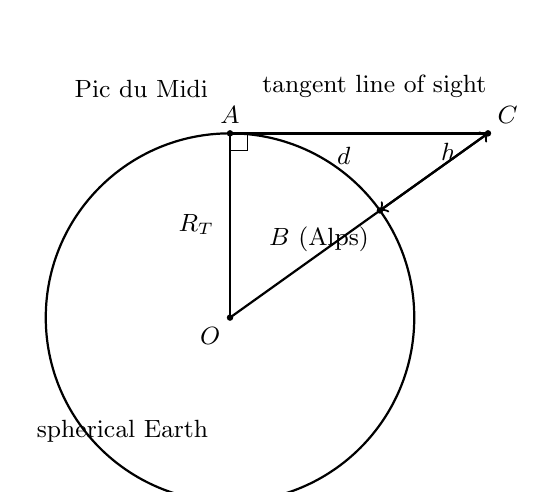
\begin{tikzpicture}[scale=0.78, every node/.style={font=\small}]
  \coordinate (O) at (0,0);
  \coordinate (A) at (0,3);
  \coordinate (C) at (4.2,3);
  \coordinate (B) at (2.441,1.744);
  \draw[thick] (O) circle (3);
  \draw[thick] (O)--(A);
  \draw[thick] (O)--(C);
  \draw[very thick] (A)--(C);
  \draw[<->,thick] (B)--(C);
  \draw (0,2.72)--(0.28,2.72)--(0.28,3);
  \fill (O) circle (1.5pt) node[below left] {$O$};
  \fill (A) circle (1.5pt) node[above] {$A$};
  \fill (B) circle (1.5pt);
  \fill (C) circle (1.5pt) node[above right] {$C$};
  \node[above left] at (-0.20,3.42) {Pic du Midi};
  \node[above] at (2.35,3.42) {tangent line of sight};
  \node[below] at (1.85,2.94) {$d$};
  \node[left] at (-0.10,1.52) {$\RT$};
  \node[above right] at (3.28,2.40) {$h$};
  \node[below left] at (2.42,1.63) {$B$ (Alps)};
  \node at (-1.75,-1.85) {spherical Earth};
\end{tikzpicture}
\caption{Tangent-horizon geometry. To the accuracy required here the map
separation is identified with the tangent length $AC$.}
\end{figure}

The triangle $OAC$ is right-angled at $A$, because $AC$ is tangent at $A$. With
$OA=\RT$, $OC=\RT+h$ and $AC\simeq d$, Pythagoras gives
\[
 (\RT+h)^2=\RT^2+d^2,
 \qquad\text{so}\qquad
 h=\sqrt{\RT^2+d^2}-\RT=\RT\left[\sqrt{1+\left(\frac{d}{\RT}\right)^2}-1\right].
\]
Since $d/\RT\ll1$,
\[
 h\simeq \frac{d^2}{2\RT}.
\]
Reading $d$ instead as an arc length along the surface gives
$h=\RT[\sec(d/\RT)-1]$, with the same leading term $d^2/(2\RT)$; at
$d=\SI{500}{km}$ the two exact forms give \SI{19.5}{km} and \SI{19.6}{km}, so
the distinction is irrelevant at one significant figure.
With $d=\SI{500}{km}$ and $\RT=\SI{6400}{km}$,
\[
 h\simeq \frac{(\SI{5.0e5}{m})^2}{2\times \SI{6.4e6}{m}}
      \simeq \SI{2.0e4}{m}
      \simeq \SI{20}{km}.
\]

Sprites lie roughly between \SI{40}{km} and \SI{80}{km}, so they can be above this geometric horizon. Mont Blanc is only about \SI{4.8}{km} high, which is far below even the \SIrange{20}{30}{km} horizon-height estimate. In the no-refraction model, Mont Blanc is not visible from Pic du Midi at this distance.

\begin{finalanswer}
$d\sim\SI{500}{km}$ for the exam order of magnitude, giving $h\sim\SI{20}{km}$. A \SI{600}{km} distance would give $h\sim\SI{30}{km}$. Alpine sprites can be visible because they are much higher than this, but Mont Blanc cannot be seen in this simplified no-refraction geometry.
\end{finalanswer}

\subsection*{Question 3 -- Why Figure 4 proves a sprite detection}
\addcontentsline{toc}{subsection}{Question 3}

Figure 4 compares two simultaneous ISS images: a narrow-band image filtered around \SI{761}{nm} and a visible-light image. The statement gives a useful calibration: a normal lightning flash gives about 836 LSB in the visible camera but only about 30 LSB in the filtered camera. For ordinary lightning, the filtered/visible ratio is therefore only
\[
 \frac{30}{836}\simeq3.6\times10^{-2}.
\]

Now read the two colour bars of Figure 4. The visible image saturates at
836~LSB and the filtered image at 62~LSB. The visible reading is therefore
exactly the signature of one conventional lightning flash. If that flash were the
only source, the filtered camera should read about 30~LSB. It reads roughly twice
that:
\[
 \frac{62}{836}\simeq7.4\times10^{-2}\simeq2\times\frac{30}{836}.
\]
So about 30~LSB of narrow-band signal is left over once the lightning is
accounted for, and it must come from something else.

That something else has to be high. The filter is centred on \SI{761}{nm},
which is an \Otwo{} absorption band. Radiation emitted at that wavelength
\emph{below} the bulk of the atmospheric oxygen is reabsorbed on its way up, so a
tropospheric flash is strongly attenuated in this band, which is precisely why
its filtered signature is only 30~LSB while its visible signature is 836~LSB. A
source emitting above roughly \SI{40}{km} has almost no \Otwo{} left above it and
is not attenuated. The excess narrow-band signal therefore identifies an emitter
at sprite altitudes.

Two further remarks support the identification. The two images are simultaneous
and the structure appears at the same place in both, so it is not camera noise,
which would not correlate between two independent detectors. And in the filtered
image the structure is visibly more extended and more ragged than the compact
saturated core of the visible image, as expected if a diffuse high-altitude
emission is superposed on a point-like flash.

\begin{finalanswer}
The visible image reads 836~LSB, i.e. one conventional flash, but the filtered image reads 62~LSB instead of the 30~LSB that flash should give at \SI{761}{nm}. The $\sim$30~LSB excess in an \Otwo{} absorption band can only come from an emitter high enough to escape reabsorption, and the two co-located simultaneous signals rule out noise. This is a sprite detection.
\end{finalanswer}

\subsection*{Question 4 -- Gravity at ISS altitude}
\addcontentsline{toc}{subsection}{Question 4}

The statement asks for the assumptions to be specified. They are: Earth is
spherical with a spherically symmetric mass distribution; the ISS is outside it;
Earth's rotation, atmospheric drag and the fields of other bodies are neglected.

Spherical symmetry forces the field to be radial with a magnitude depending only
on $r$,
\[
 \mathbf g(r)=-g(r)\,\mathbf e_r,
\]
so $g$ is constant over any sphere $\mathcal S_r$ centred on Earth. Gauss'
theorem for gravitation, the analogue of the electrostatic one with
$1/\varepsilon_0\to-4\pi G_N$, reads
\[
 \oint_{\mathcal S_r}\mathbf g\cdot d\mathbf S=-4\pi G_N M_T .
\]
With $d\mathbf S$ outward, the left-hand side is $-g(r)\,4\pi r^2$, hence
\[
 g(r)=\frac{G_N M_T}{r^2}.
\]
This is the standard result that a spherically symmetric body acts, on the
outside, like a point mass at its centre. Applying it twice, at $r=\RT$ and at
$r=\RT+h_{\ISS}$ with $h_{\ISS}\simeq\SI{400}{km}$,
\[
 g_0=\frac{G_N M_T}{\RT^2},
 \qquad
 G_{\ISS}=\frac{G_N M_T}{(\RT+h_{\ISS})^2},
\]
and dividing the second by the first:
\[
 G_{\ISS}=g_0\left(\frac{\RT}{\RT+h_{\ISS}}\right)^2
          =g_0\left(1+\frac{h_{\ISS}}{\RT}\right)^{-2}.
\]
Numerically,
\[
 \frac{h_{\ISS}}{\RT}=\frac{400}{6400}=0.0625,
\]
so
\[
 G_{\ISS}=\frac{9.8}{(1.0625)^2}\simeq\SI{8.7}{m.s^{-2}}.
\]

\begin{finalanswer}
\[
G_{\ISS}=g_0\left(1+\frac{h_{\ISS}}{\RT}\right)^{-2}\simeq\SI{9}{m.s^{-2}}.
\]
\end{finalanswer}

\subsection*{Question 5 -- ISS orbital speed}
\addcontentsline{toc}{subsection}{Question 5}

The statement says ``after showing that it is constant'', so this has to be
proved rather than assumed. On a circular orbit the velocity is tangential while
the gravitational field is radial, so the two are orthogonal and
\[
 \frac{d}{dt}\!\left(\frac{v^2}{2}\right)
 =\mathbf v\cdot\frac{d\mathbf v}{dt}
 =\mathbf v\cdot\mathbf g=0 .
\]
The speed $v_{\ISS}$ is therefore constant: gravity does no work here, it only
turns the velocity.

Writing $r=\RT+h_{\ISS}$, a uniform circular motion has purely centripetal
acceleration, and Newton's second law projected on $\mathbf e_r$ gives
\[
 \mathbf a=-\frac{v_{\ISS}^2}{r}\,\mathbf e_r=\mathbf g=-G_{\ISS}\,\mathbf e_r,
 \qquad\text{so}\qquad
 \frac{v_{\ISS}^2}{r}=G_{\ISS}.
\]
Thus
\[
 v_{\ISS}=\sqrt{G_{\ISS}(\RT+h_{\ISS})}.
\]
Using the expression from Question 4,
\[
 v_{\ISS}=\sqrt{\frac{g_0\RT^2}{\RT+h_{\ISS}}}.
\]
Numerically,
\[
 v_{\ISS}\simeq\sqrt{\frac{9.8(\SI{6.4e6}{m})^2}{\SI{6.8e6}{m}}}
 \simeq \SI{7.7e3}{m.s^{-1}}.
\]

\begin{finalanswer}
The speed is constant because the force is radial and the velocity tangential, so $\mathbf v\cdot\mathbf g=0$. Then
\[
v_{\ISS}=\sqrt{\frac{g_0\RT^2}{\RT+h_{\ISS}}}\simeq\SI{8}{km.s^{-1}}.
\]
\end{finalanswer}

\subsection*{Question 6 -- ISS period and Kepler's third law}
\addcontentsline{toc}{subsection}{Question 6}

One circular orbit has length $2\pi(\RT+h_{\ISS})$. Therefore
\[
 T_{\ISS}=\frac{2\pi(\RT+h_{\ISS})}{v_{\ISS}}.
\]
Substitute the speed from Question 5:
\[
 T_{\ISS}=2\pi\sqrt{\frac{(\RT+h_{\ISS})^3}{g_0\RT^2}}.
\]
Since $g_0\RT^2=G M_T$, this is also
\[
 T_{\ISS}=2\pi\sqrt{\frac{r^3}{G M_T}},\qquad r=\RT+h_{\ISS}.
\]
Squaring,
\[
 T_{\ISS}^2=\frac{4\pi^2}{G M_T}r^3.
\]
This is Kepler's third law: $T^2$ is proportional to $r^3$.

Numerically,
\[
 T_{\ISS}\simeq \frac{2\pi(\SI{6.8e6}{m})}{\SI{7.7e3}{m.s^{-1}}}
 \simeq\SI{5.6e3}{s}
 \simeq\SI{93}{min}.
\]

\begin{finalanswer}
\[
T_{\ISS}\simeq\SI{90}{min},\qquad T^2\propto r^3.
\]
\end{finalanswer}

\subsection*{Question 7 -- Can the ISS cameras record a whole sprite?}
\addcontentsline{toc}{subsection}{Question 7}

The axes of Figure 4 give the field of view directly: about \SI{22}{km}
horizontally by \SI{20}{km} vertically.

The cameras point at nadir, so the field sweeps across the emitting layer at the
\emph{ground-track} speed rather than at the orbital speed. For a target at
altitude $z$,
\[
 v_{\rm sweep}=v_{\ISS}\,\frac{R_T+z}{R_T+h_{\ISS}}
 \simeq\SI{7.7}{km.s^{-1}}\times\frac{6460}{6800}
 \simeq\SI{7.3}{km.s^{-1}}
\]
at $z=\SI{60}{km}$. The difference from $v_{\ISS}$ is only about 5\,\%, so at one
significant figure it changes nothing. The time to cross the field is
\[
 \Delta t_{\rm field}\simeq \frac{\SI{20}{km}}{\SI{7}{km.s^{-1}}}\simeq\SI{3}{s}.
\]
A sprite lasts only a few hundred milliseconds. For example,
\[
\SI{0.1}{s}\Rightarrow \Delta x\simeq\SI{0.8}{km},
\qquad
\SI{0.3}{s}\Rightarrow \Delta x\simeq\SI{2.4}{km}.
\]
These distances are much smaller than the \SI{20}{km} field of view, so recording the whole event is possible if the storm lies inside the field at the right time.

For precision, the image scale is roughly
\[
 \frac{\SI{20}{km}}{40\text{--}50\text{ pixels}}\simeq \SIrange{0.4}{0.5}{km/pixel}.
\]
The ISS also moves by about a kilometre during a typical event. So the natural spatial precision is not metres; it is about a kilometre.

\begin{finalanswer}
Recording a whole sprite is possible: the field is crossed in about \SIrange{2.5}{3}{s}, while the sprite lasts only a few \SI{0.1}{s}. The spatial precision is roughly kilometre-scale, set both by the pixel size ($\sim\SI{0.45}{km}$) and by the $\sim\SI{1}{km}$ of ISS motion during the event. The real limitation is not the timing but the coincidence: the storm must lie inside a \SI{20}{km} window during the few seconds of the pass. The temporal resolution itself cannot be quantified from the statement, since neither the frame rate nor the exposure time is given.
\end{finalanswer}

\subsection*{Part I (continued) -- A variable-pressure atmosphere}\addcontentsline{toc}{section}{Part I (continued) -- A variable-pressure atmosphere}

\subsection*{Question 8 -- Hydrostatic equation and scale height}
\addcontentsline{toc}{subsection}{Question 8}

The vector law of hydrostatic equilibrium is
\[
 \grad P=\mu\,\mathbf{g},
\]
where $\mu$ is the mass density and $\mathbf{g}$ points downward. If $z$ is upward, this becomes
\[
 \frac{dP}{dz}=-\mu g(z).
\]

The atmosphere is treated as an ideal gas. For molar mass $M$,
\[
 \mu=\frac{PM}{RT(z)}.
\]
The temperature model is
\[
 T(z)=T_0\left(1-\frac{z}{\ell}\right),
\]
and gravity is
\[
 g(z)=g_0\left(1+\frac{z}{\RT}\right)^{-2}.
\]
Therefore
\[
 \frac{dP}{dz}
 =-\frac{PM}{RT_0(1-z/\ell)}g_0\left(1+\frac{z}{\RT}\right)^{-2}.
\]
Define the characteristic height
\[
 H=\frac{RT_0}{Mg_0}.
\]
Then
\[
 \frac{dP}{dz}=-F(z)\frac{P}{H},
 \qquad
 F(z)=\frac{1}{(1-z/\ell)(1+z/\RT)^2}.
\]

Numerically, with $T_0=\SI{290}{K}$ and $M=\SI{29e-3}{kg.mol^{-1}}$,
\[
 H=\frac{8.31\times 290}{0.029\times9.8}=\SI{8.48e3}{m}=\SI{8.5}{km}.
\]
Rounded to the single significant figure requested by the statement,
\[
 H\simeq\SI{8}{km}.
\]
(The unrounded value \SI{8.5}{km} is the one to keep for the later numerical
work in Questions 9 and 10.)

\begin{finalanswer}
\[
\frac{dP}{dz}=-F(z)\frac{P}{H},\qquad
F(z)=\frac{1}{(1-z/\ell)(1+z/\RT)^2},\qquad
H=\frac{RT_0}{Mg_0}=\SI{8.5}{km}\simeq\SI{8}{km}.
\]
\end{finalanswer}

\subsection*{Question 9 -- Pressure law}
\addcontentsline{toc}{subsection}{Question 9}

The statement gives a decomposition
\[
F(z)=\frac{\alpha}{1-z/\ell}+\frac{\beta+\gamma z}{(1+z/\RT)^2},
\]
with $\varepsilon=\ell/\RT$. The exact coefficients can be written more compactly,
since $1+\varepsilon(2+\varepsilon)=(1+\varepsilon)^2$:
\[
 \alpha=\frac{1}{(1+\varepsilon)^2},
 \qquad
 \beta=\frac{\varepsilon(2+\varepsilon)}{(1+\varepsilon)^2},
 \qquad
 \gamma=\frac{\alpha\varepsilon}{\RT}.
\]
Here
\[
 \varepsilon=\frac{50}{6400}=7.8\times10^{-3}\ll1,
\]
so $(1+\varepsilon)^2=1+1.6\times10^{-2}$ and, to first order in $\varepsilon$,
\[
\alpha\simeq1,
\qquad
\beta\simeq2\varepsilon,
\qquad
\gamma\simeq\frac{\varepsilon}{\RT}.
\]
The error committed is of order $2\varepsilon\simeq1.6\,\%$ on $\alpha$ and
$\beta$, far below the one-significant-figure precision requested.

The pressure equation is
\[
 \frac{dP}{P}=-\frac{F(z)}{H}\,dz.
\]
Integrate from $0$ to $z$, using $P(0)=P_0$.

First term:
\[
 \int_0^z \frac{du}{1-u/\ell}
 =-\ell\ln\left(1-\frac{z}{\ell}\right).
\]
This gives the factor
\[
 \left(1-\frac{z}{\ell}\right)^{\ell/H}.
\]

For the second term, with $y=1+u/\RT$, one obtains
\[
\int_0^z \frac{2\varepsilon+(\varepsilon/\RT)u}{(1+u/\RT)^2}\,du
=\ell\left[\ln\left(1+\frac{z}{\RT}\right)+1-\frac{1}{1+z/\RT}\right].
\]
Here we used $\varepsilon\RT=\ell$. Also,
\[
1-\frac{1}{1+z/\RT}=\frac{z/\RT}{1+z/\RT}.
\]
So, after multiplication by $-1/H$, the non-logarithmic part contributes
\[
-\frac{\ell}{H}\frac{z/\RT}{1+z/\RT}
=-\frac{z}{(H\RT/\ell)(1+z/\RT)}.
\]
This gives both a denominator power of $1+z/\RT$ and a small exponential correction.

Thus
\[
P(z)=P_0
\left(\frac{1-z/\ell}{1+z/\RT}\right)^{\xi}
\exp\left[-\frac{z}{\chi(1+z/\RT)}\right],
\]
where
\[
 \xi=\frac{\ell}{H},
 \qquad
 \chi=\frac{H\RT}{\ell}.
\]
Numerically,
\[
 \xi\simeq\frac{50}{8.5}\simeq 5.9\simeq6,
 \qquad
 \chi\simeq\frac{8.5\times6400}{50}\,\si{km}\simeq\SI{1.1e3}{km}.
\]

\begin{finalanswer}
\[
P(z)=P_0
\left(\frac{1-z/\ell}{1+z/\RT}\right)^{\ell/H}
\exp\left[-\frac{z}{(H\RT/\ell)(1+z/\RT)}\right].
\]
So $\xi=\ell/H$ and $\chi=H\RT/\ell$.
\end{finalanswer}

\subsection*{Question 10 -- Useful simplification of the pressure law}
\addcontentsline{toc}{subsection}{Question 10}

For altitudes below \SI{50}{km}, the ratio $z/\RT$ is tiny:
\[
 \frac{50}{6400}\simeq 8\times10^{-3}.
\]
So
\[
 1+\frac{z}{\RT}\simeq 1.
\]
Also $\chi\simeq\SI{1100}{km}$, so
\[
 \exp\left[-\frac{z}{\chi(1+z/\RT)}\right]\simeq 1
\]
for $z\leq\SI{50}{km}$.

Therefore the practical simplified pressure law is
\[
 P(z)\simeq P_0\left(1-\frac{z}{\ell}\right)^{\ell/H}.
\]
This simplification amounts to neglecting the variation of gravity with altitude while keeping the imposed temperature law.

At very low altitude, if $z\ll\ell$, one can go further:
\[
 \left(1-\frac{z}{\ell}\right)^{\ell/H}
 \simeq \exp\left(-\frac{z}{H}\right),
\]
which is the familiar exponential barometric law.

\begin{finalanswer}
\[
P(z)\simeq P_0\left(1-\frac{z}{\ell}\right)^{\ell/H}.
\]
This keeps the temperature decrease but neglects Earth-curvature / gravity variation.
\end{finalanswer}

\subsection*{Question 11 -- Why the model fails near \SI{20}{km}}
\addcontentsline{toc}{subsection}{Question 11}

The model was built with the temperature law
\[
 T(z)=T_0\left(1-\frac{z}{\ell}\right),\qquad \ell=\SI{50}{km}.
\]
This is a linear decrease at a fixed rate $T_0/\ell=\SI{5.8}{K.km^{-1}}$, which is
a reasonable description of the troposphere and nothing else. The real
atmosphere stops cooling at the tropopause, around \SIrange{10}{15}{km}, and then
\emph{warms} through the stratosphere because ozone absorbs solar ultraviolet.
The numbers make the failure obvious:
\[
 T_{\rm model}(\SI{20}{km})=290\times0.6=\SI{174}{K}
 \quad\text{against}\quad
 T_{\rm real}\simeq\SI{217}{K},
\]
\[
 T_{\rm model}(\SI{50}{km})=\SI{0}{K}
 \quad\text{against}\quad
 T_{\rm real}\simeq\SI{270}{K}.
\]
Too low a temperature means too small a local scale height $RT(z)/(Mg)$, hence a
pressure that falls too fast. This is exactly what Figure 5 shows: the dashed
model curve follows the measurement up to about \SI{20}{km}, then bends away
below it and collapses vertically at $z=\ell=\SI{50}{km}$, where the model
temperature reaches absolute zero and the factor $(1-z/\ell)^{\xi}$ vanishes.

\begin{finalanswer}
The linear temperature law is a troposphere-only model. Above the tropopause ($\sim$\SIrange{10}{15}{km}) the real temperature stops falling and then rises, while the model keeps cooling to \SI{0}{K} at $z=\ell$. The model temperature is therefore far too low, the scale height too small, and the predicted pressure collapses well below the measured one from about \SI{20}{km} upward.
\end{finalanswer}

\subsection*{Question 12 -- Observation from Earth and from the ISS}
\addcontentsline{toc}{subsection}{Question 12}

The oxygen molar fraction is assumed constant:
\[
 x_{\Otwo}\simeq 0.20.
\]
Therefore the oxygen partial pressure is
\[
 P_{\Otwo}(z)=x_{\Otwo}P(z)\simeq0.20P(z).
\]
so the oxygen profile has the same shape as the pressure profile. Two numbers
are enough. At the ground,
\[
 P_{\Otwo}(0)=0.20\times\SI{1}{bar}=\SI{2e4}{Pa}.
\]
At \SI{60}{km} the model of Question 9 must not be used: Question 11 showed it is
no longer quantitatively reliable there, and in any case $z=\SI{60}{km}$ lies
beyond its domain $z<\ell$. The measured value supplied by Question 20 is used
instead, $P_3=\SI{20}{Pa}$, so
\[
 P_{\Otwo}(\SI{60}{km})=0.20\times20=\SI{4}{Pa},
\]
smaller by a factor $5\times10^{3}$.

What matters for absorption is not the local partial pressure but the total
amount of \Otwo{} \emph{along the line of sight}. A ground observer looking up at
a sprite sees it through the whole oxygen column, essentially all of which lies
below \SI{20}{km}; at \SI{762}{nm} this column is optically thick, which is why
the transmission notch in Figure 2 reaches zero.

From the ISS the geometry is reversed. The camera is at \SI{400}{km} and the
source is at \SIrange{40}{80}{km}, so the light only has to cross the atmosphere
\emph{above} the source, where the residual pressure is a few pascals or less,
i.e. thousands of times thinner than at the ground and containing a negligible
\Otwo{} column. The \SI{761}{nm} band is then transparent, which is exactly why
this filter can be used from orbit as a sprite discriminator (Question 3) and
could not be used from the ground.

\begin{finalanswer}
From the ground the line of sight crosses the entire \Otwo{} column, from \SI{4}{Pa} of partial pressure at \SI{60}{km} up to \SI{2e4}{Pa} at the surface, and the \SI{762}{nm} band is opaque. From the ISS the light only crosses the atmosphere above the sprite, where the \Otwo{} column is negligible, so the same band becomes usable and even diagnostic.
\end{finalanswer}

\section{Part II -- An electrical atmosphere}

\subsection*{Question 13 -- Neglecting the magnetic Lorentz force}
\addcontentsline{toc}{subsection}{Question 13}

The Lorentz force on an electron is
\[
 \mathbf{F}=q(\E+\mathbf{v}\times\B).
\]
The relation between $\B$ and $\E$ should be taken from Faraday's law rather than
assumed to be $B=E/c$: the plasma is dispersive, so its phase velocity is not
$c$. For the plane wave $\E=\E_0e^{i(\omega t-kz)}$,
\[
 \B=\frac{k}{\omega}\,\mathbf e_z\times\E,
 \qquad\text{so}\qquad
 B=\frac{E}{v_\varphi},
 \qquad v_\varphi=\frac{\omega}{k}.
\]
The ratio of the two contributions to the Lorentz force is therefore
\[
 \frac{|q\mathbf{v}\times\B|}{|q\E|}\leq\frac{vB}{E}=\frac{v}{v_\varphi}.
\]
The dispersion relation of Question 15 gives $v_\varphi\geq c$ for any
propagating mode, so this bound is even tighter than $v/c$. The statement
specifies non-relativistic electrons, $v\ll c\leq v_\varphi$, and the magnetic
term is negligible.

The estimate is self-consistent with Question 14, which gives $v=eE/(m_e\omega)$
for the velocity driven by the wave:
\[
 \frac{v}{v_\varphi}\leq\frac{v}{c}=\frac{eE}{m_e\omega c},
\]
which stays $\ll1$ for any field amplitude and frequency of interest here: at
$\omega\sim10^{7}\,\mathrm{rad\,s^{-1}}$ it would take
$E\sim10^{9}\,\mathrm{V\,m^{-1}}$ to reach $v\sim c$, far above the
$\SI{100}{V.m^{-1}}$ scale quoted later in the statement.

\begin{finalanswer}
With $\B=(k/\omega)\,\mathbf e_z\times\E$, the magnetic contribution is smaller than the electric one by a factor $v/v_\varphi\leq v/c\ll1$, so it is negligible.
\end{finalanswer}

\subsection*{Question 14 -- Electron current and plasma conductivity}
\addcontentsline{toc}{subsection}{Question 14}

Under a harmonic field, a carrier of charge $q$ and mass $m$ reaches a velocity
amplitude $|q|E/(m\omega)$, so its current density scales as $nq^2E/(m\omega)$. In
a quasi-neutral, singly ionized plasma $n_i\simeq n_e$ and the charges are equal
in magnitude, so the two currents differ only by the mass ratio:
\[
 \left|\frac{j_i}{j_e}\right|\simeq\frac{m_e}{m_i}\lesssim10^{-4},
\]
since even a proton is about $1800$ times heavier than an electron, and
atmospheric ions are heavier still. The ion current is therefore negligible.

Let $e>0$ be the elementary charge; an electron has charge $-e$. The equation of motion is
\[
 m_e\frac{d\mathbf{v}}{dt}=-e\E.
\]
The field has complex time dependence $\exp(i\omega t)$, so $d/dt$ becomes $i\omega$:
\[
 i\omega m_e\mathbf{v}=-e\E.
\]
Therefore
\[
 \mathbf{v}=\frac{i e}{m_e\omega}\E.
\]
The electron current density is
\[
 \jv=n(-e)\mathbf{v}.
\]
Thus
\[
 \jv=-i\frac{n e^2}{m_e\omega}\E.
\]
By definition, $\jv=\gamma_p\E$, so
\[
 \gamma_p=-i\frac{n e^2}{m_e\omega}.
\]
This conductivity is purely imaginary, which has a direct energetic meaning. For
complex amplitudes the cycle-averaged power density delivered to the medium is
\[
 \langle p\rangle=\frac12\operatorname{Re}\left(\jv_0\cdot\E_0^{*}\right)
 =\frac12\operatorname{Re}(\gamma_p)\,|\E_0|^2=0 ,
\]
because $\operatorname{Re}(\gamma_p)=0$. The conductivity is purely reactive: with
no collisions the plasma exchanges energy back and forth with the wave over a
cycle but dissipates none on average. Equivalently, the velocity is in quadrature
with the field, so the force does no net work.

\begin{finalanswer}
\[
\gamma_p=-i\frac{n e^2}{m_e\omega}.
\]
It is purely imaginary, so the average absorbed power is zero in this collisionless model.
\end{finalanswer}

\subsection*{Question 15 -- Wave equation and dispersion relation}
\addcontentsline{toc}{subsection}{Question 15}

Use Maxwell's equations in a plasma with current density $\jv$:
\[
 \nabla\times\B=\mu_0\jv+\mu_0\varepsilon_0\frac{\partial\E}{\partial t},
 \qquad
 \nabla\times\E=-\frac{\partial\B}{\partial t}.
\]
Before combining them, note that $\nabla\cdot\E=0$ here. For the wave specified in
the statement this is immediate, since $\E_0\perp\mathbf e_z$ gives
\[
 \nabla\cdot\E=-ik\,\mathbf e_z\cdot\E=0 .
\]
It is worth checking that this is dynamically consistent rather than merely
assumed. Charge conservation and Gauss' law give
\[
 \frac{\partial\rho}{\partial t}+\nabla\cdot\jv=0,
 \qquad
 \nabla\cdot\E=\frac{\rho}{\varepsilon_0},
 \qquad
 \jv=\gamma_p\E,
\]
so $i\omega\rho+\gamma_p\rho/\varepsilon_0=0$. With
$\gamma_p=-i\,ne^2/(m_e\omega)$ this reads
\[
 i\rho\left(\omega-\frac{\omega_p^2}{\omega}\right)=0,
\]
which forces $\rho=0$ unless $\omega=\omega_p$. The medium therefore stays
locally neutral and the wave is transverse.

Taking the curl of Faraday's law and using $\nabla\cdot\E=0$ gives
\[
 \Delta\E-\mu_0\varepsilon_0\frac{\partial^2\E}{\partial t^2}
 =\mu_0\frac{\partial\jv}{\partial t}.
\]
Since $c^2=1/(\mu_0\varepsilon_0)$,
\[
 \Delta\E-\frac{1}{c^2}\frac{\partial^2\E}{\partial t^2}
 =\mu_0\frac{\partial\jv}{\partial t}.
\]

Insert
\[
 \E=\E_0e^{i(\omega t-kz)},\qquad \jv=\gamma_p\E.
\]
Then $\Delta\to -k^2$ and $\partial_t\to i\omega$, so
\[
 -k^2+\frac{\omega^2}{c^2}=\mu_0 i\omega\gamma_p.
\]
Using $\gamma_p=-i n e^2/(m_e\omega)$,
\[
 -k^2+\frac{\omega^2}{c^2}=\mu_0\frac{n e^2}{m_e}.
\]
Since $\mu_0=1/(\varepsilon_0c^2)$,
\[
 k^2=\frac{\omega^2-\omega_p^2}{c^2},
 \qquad
 \omega_p^2=\frac{n e^2}{m_e\varepsilon_0}.
\]

\begin{finalanswer}
\[
\omega^2=\omega_p^2+c^2k^2,
\qquad
\omega_p^2=\frac{n e^2}{m_e\varepsilon_0}.
\]
\end{finalanswer}

\subsection*{Question 16 -- Plasma cutoff frequency}
\addcontentsline{toc}{subsection}{Question 16}

For propagation, the wave number $k$ must be real. Since
\[
 k^2=\frac{\omega^2-\omega_p^2}{c^2},
\]
we need
\[
 \omega>\omega_p.
\]
If $\omega<\omega_p$, then $k^2<0$, $k$ is imaginary, and the wave is evanescent: it cannot propagate through that plasma region.

The cutoff frequency is
\[
 f_p=\frac{\omega_p}{2\pi}
 =\frac{1}{2\pi}\sqrt{\frac{n e^2}{m_e\varepsilon_0}}.
\]
For $n=\SI{1e11}{m^{-3}}$,
\[
 \omega_p=\sqrt{\frac{(10^{11})(1.60\times10^{-19})^2}{(9.11\times10^{-31})(8.85\times10^{-12})}}
 \simeq\SI{1.8e7}{rad.s^{-1}}.
\]
Therefore
\[
 f_p=\frac{1.8\times10^7}{2\pi}\simeq\SI{2.8e6}{Hz}\simeq\SI{3}{MHz}.
\]

\begin{finalanswer}
\[
f_p\simeq\SI{3}{MHz}\quad\text{for}\quad n=\SI{1e11}{m^{-3}}.
\]
Waves below this frequency cannot propagate through such a dense plasma.
\end{finalanswer}

\subsection*{Question 17 -- Interpreting the \SI{2.2}{MHz} radar map}
\addcontentsline{toc}{subsection}{Question 17}

A radar echo returns when the wave is reflected. In this plasma model, reflection happens when the local plasma frequency is at least the radar frequency.

For $f=\SI{2.2}{MHz}$, the electron density needed for cutoff is
\[
 n_{\rm cut}=\frac{m_e\varepsilon_0(2\pi f)^2}{e^2}.
\]
Numerically,
\[
 n_{\rm cut}\simeq\SI{6e10}{m^{-3}}.
\]
This is close to the sprite characteristic density $\SI{1e11}{m^{-3}}$ found in Question 16.

This is the key point: the density needed to turn back a \SI{2.2}{MHz} wave is
of the same order as the sprite density $\SI{1e11}{m^{-3}}$ used in Question 16,
and about $10^{4}$ times the ambient night-time density of the D~region near
\SI{60}{km}. Any echo coming from that altitude therefore requires ionization
that is not normally there.

Figure 6 shows two distinct things.
\begin{itemize}[nosep]
\item A permanent, horizontally continuous reflecting layer above about
\SI{95}{km}, with the strongest amplitudes beyond \SI{100}{km}. This is simply
the bottom of the ionosphere and is present throughout the record.
\item Narrow, quasi-vertical columns that appear only at two instants of the
record and reach down to \SIrange{50}{60}{km}, with local amplitude maxima
(the highest amplitude class) near \SIrange{55}{65}{km} and
\SIrange{70}{85}{km}.
\end{itemize}
Their transient character in time, their small horizontal extent, and their
altitude range, which coincides with the \SIrange{40}{80}{km} band where sprites
occur, all point the same way: these are localized, short-lived patches of
ionization created by high-altitude discharges, not permanent ionospheric
structure. This is an independent, radio-frequency confirmation of the optical
detections of Part~I.

A remark on the figure itself: the horizontal axis is labelled as the delay
between the radar pulse and its echo, in seconds, but a reflection at
\SIrange{50}{110}{km} corresponds to a two-way delay of only
\SIrange{0.3}{0.7}{ms}. The vertical axis already carries that delay, converted
into a reflection height. The horizontal axis must therefore be the elapsed
observation time within the record; the label appears to be an error in the
original document.

\begin{finalanswer}
The \SI{2.2}{MHz} radar reflects only where $n_e\gtrsim\SI{6e10}{m^{-3}}$, comparable to the sprite density of Question 16 and far above the ambient value at these altitudes. The permanent layer above \SI{95}{km} is the ionosphere; the transient columns reaching down to \SIrange{50}{60}{km} are localized patches of ionization produced by sprite-related discharges.
\end{finalanswer}

\section{Part III -- Avalanche formation of a current}

\subsection*{Question 18 -- Survival equation before collision}
\addcontentsline{toc}{subsection}{Question 18}

Consider a slice between $x$ and $x+dx$. Its volume is
\[
 \Sigma\,dx.
\]
If the molecule number density is $n_{\rm mo}$, the number of molecules in the slice is
\[
 n_{\rm mo}\Sigma\,dx.
\]
Each molecule presents an effective collision cross-section $S_{\rm eff}$. The total effective area in the slice is therefore
\[
 n_{\rm mo}\Sigma\,dx\,S_{\rm eff}.
\]
Dividing by the total section $\Sigma$, the probability that an electron collides in this slice is
\[
 n_{\rm mo}S_{\rm eff}\,dx.
\]

If $N(x)$ electrons have reached $x$ without collision, the number lost in the next slice is
\[
 dN=-N(x)n_{\rm mo}S_{\rm eff}\,dx.
\]
So
\[
 \frac{dN}{dx}=-n_{\rm mo}S_{\rm eff}N.
\]
Solving with $N(0)=N_0$,
\[
 N(x)=N_0\exp(-n_{\rm mo}S_{\rm eff}x).
\]

\begin{finalanswer}
\[
\frac{dN}{dx}=-n_{\rm mo}S_{\rm eff}N,
\qquad
N(x)=N_0\exp(-n_{\rm mo}S_{\rm eff}x).
\]
\end{finalanswer}

\subsection*{Question 19 -- Mean free path}
\addcontentsline{toc}{subsection}{Question 19}

The quantity asked for is a \emph{mean}, so it has to be obtained from the
distribution of free paths, not merely by reading off the decay constant of
$N(x)$.

Write $a=n_{\rm mo}S_{\rm eff}$, so that $N(x)=N_0e^{-ax}$. Among the $N_0$
electrons, those undergoing their first collision between $x$ and $x+dx$ are the
ones lost from $N$ over that slice:
\[
 dN_{\rm coll}=-dN=N_0\,a\,e^{-ax}\,dx.
\]
The probability density of the free path is therefore
\[
 p(x)=\frac{1}{N_0}\frac{dN_{\rm coll}}{dx}=a\,e^{-ax},
 \qquad x\geq0,
\]
which is correctly normalised: $\int_0^{\infty}a e^{-ax}dx=1$. The mean free path
is then
\[
 \ell_{pm}=\langle x\rangle=\int_0^{\infty}x\,p(x)\,dx
 =a\int_0^{\infty}x\,e^{-ax}\,dx.
\]
Integrating by parts,
\[
 \int_0^{\infty}x\,e^{-ax}\,dx
 =\left[-\frac{x}{a}e^{-ax}\right]_0^{\infty}
 +\frac{1}{a}\int_0^{\infty}e^{-ax}dx
 =0+\frac{1}{a^2},
\]
so $\langle x\rangle=a\times a^{-2}=1/a$, that is
\[
 \ell_{pm}=\frac{1}{n_{\rm mo}S_{\rm eff}}.
\]

Equivalently, and faster, one may integrate the survival function directly:
$\langle x\rangle=\int_0^{\infty}\bigl(N(x)/N_0\bigr)dx=\int_0^{\infty}e^{-ax}dx=1/a$.

\begin{finalanswer}
\[
\ell_{pm}=\frac{1}{n_{\rm mo}S_{\rm eff}}.
\]
\end{finalanswer}

\subsection*{Question 20 -- Mean free path at \SI{60}{km}}
\addcontentsline{toc}{subsection}{Question 20}

The value $S_{\rm eff}\sim\SI{1e-20}{m^2}$ is reasonable because a molecule has a size of order \SI{1e-10}{m}; an area is therefore of order
\[
 (10^{-10})^2=10^{-20}\,\mathrm{m^2}.
\]

Use the ideal gas law in number-density form:
\[
 n_{\rm mo}=\frac{P}{k_BT}.
\]
At \SI{60}{km}, the statement gives $P_3=\SI{20}{Pa}$ and $T_3=\SI{260}{K}$, so
\[
 n_{\rm mo}=\frac{20}{(1.38\times10^{-23})\times260}
 \simeq\SI{5.6e21}{m^{-3}}.
\]
Then
\[
 \ell_{pm}=\frac{1}{(5.6\times10^{21})(10^{-20})}
 \simeq\SI{1.8e-2}{m}.
\]

\begin{finalanswer}
\[
\ell_{pm}\simeq\SI{2e-2}{m}\simeq\SI{2}{cm}.
\]
\end{finalanswer}

\subsection*{Question 21 -- Can a resting electron ionize nitrogen?}
\addcontentsline{toc}{subsection}{Question 21}

The electric field is $E\simeq\SI{100}{V.m^{-1}}$. Over one mean free path, the potential difference is
\[
 \Delta V=E\ell_{pm}\simeq 100\times0.018\simeq\SI{1.8}{V}.
\]
An electron crossing a potential difference of \SI{1.8}{V} gains \SI{1.8}{eV}. The ionization energy of nitrogen is
\[
 \mathcal{E}_i\simeq\SI{16}{eV}.
\]
So the typical energy gained before a collision is far too small.

The distance needed to gain \SI{16}{eV} is
\[
 x_i=\frac{16\,\mathrm{V}}{\SI{100}{V.m^{-1}}}=\SI{0.16}{m}.
\]
In units of the mean free path,
\[
 \frac{x_i}{\ell_{pm}}\simeq\frac{0.16}{0.018}\simeq 9.
\]
The probability of travelling that far without collision is roughly $e^{-9}\sim10^{-4}$. Such a long free path is possible, but rare.

\begin{finalanswer}
A resting electron typically gains only about \SI{2}{eV} before collision, much less than \SI{16}{eV}. It will not normally ionize \Ntwo; only rare paths of about nine mean free paths, with probability $e^{-9}\sim10^{-4}$, could do it.
\end{finalanswer}

\subsection*{Question 22 -- Why \SI{1}{MeV} cosmic electrons are relativistic}
\addcontentsline{toc}{subsection}{Question 22}

The rest energy of an electron is
\[
 m_e c^2\simeq\SI{0.511}{MeV}.
\]
A kinetic energy of \SI{1}{MeV} is about twice the rest energy, so the
non-relativistic approximation cannot be valid. The cleanest way to show that it
is \emph{necessarily} invalid is to assume the opposite and reach a
contradiction: with $K=\tfrac12 m_ev^2$,
\[
 v=\sqrt{\frac{2K}{m_e}}
  =\sqrt{\frac{2\times1\times10^{6}\times1.60\times10^{-19}}{9.11\times10^{-31}}}
  \simeq\SI{5.9e8}{m.s^{-1}}\simeq2c,
\]
which is impossible. A \SI{1}{MeV} electron must therefore be treated
relativistically.

The Lorentz factor is
\[
 \Gamma=1+\frac{K}{m_e c^2}
 \simeq1+\frac{1}{0.511}
 \simeq2.96\simeq3.
\]
Then
\[
 \frac{v}{c}=\sqrt{1-\frac{1}{\Gamma^2}}
 \simeq0.94.
\]

\begin{finalanswer}
A \SI{1}{MeV} electron has $\Gamma\simeq3$ and $v\simeq0.94c$, so it is necessarily relativistic.
\end{finalanswer}

\subsection*{Question 23 -- Cascade avalanche explanation}
\addcontentsline{toc}{subsection}{Question 23}

A high-energy primary electron can ionize a nitrogen molecule during a collision. That collision releases a secondary electron. After the first ionization, there are more free electrons than before. These electrons can themselves be accelerated and produce more ionizations.

Fix the counting convention that Question 24 will use: one primary electron is
present at stage $0$, and an impact ionization leaves the incident electron free
while releasing one new electron from the molecule, so an ideal stage doubles the
population:
\[
 1\to2\to4\to8\to\cdots,
 \qquad
 N_e(\mathcal{N})\simeq2^{\mathcal{N}} .
\]
This is exponential growth. The energy is supplied by the electric field, which
re-accelerates every electron between two collisions, and by the energetic
primary particle. The process is called an avalanche because each generation creates more particles able to create the next generation.

The avalanche cannot grow forever. It can be limited by energy losses, recombination, attachment to neutral molecules, or screening of the electric field by the newly produced charges. During the process, excited molecules can emit visible light, which contributes to the sprite glow.

\begin{finalanswer}
A cascade avalanche is a chain reaction of impact ionizations. One energetic electron creates secondary electrons, which create more ionizations, leading to approximately exponential growth of electron number and current.
\end{finalanswer}

\subsection*{Question 24 -- Avalanche stage number}
\addcontentsline{toc}{subsection}{Question 24}

We want the average electron density to reach
\[
 n=\SI{1e11}{m^{-3}}.
\]
Let $\mathcal{N}$ be the number of avalanche stages. In a doubling model, the number of electrons after $\mathcal{N}$ stages is approximately
\[
 2^{\mathcal{N}}.
\]
The problem states that the electrons are contained in a characteristic volume
\[
 (\mathcal{N}\ell_{pm})^3.
\]
Using $\ell_{pm}\simeq\SI{2}{cm}=\SI{2e-2}{m}$ from Question 20,
\[
 n\simeq\frac{2^{\mathcal{N}}}{(\mathcal{N}\ell_{pm})^3}.
\]
Set this equal to $\SI{1e11}{m^{-3}}$:
\[
 10^{11}=\frac{2^{\mathcal{N}}}{\mathcal{N}^3(2\times10^{-2})^3}.
\]
So
\[
 2^{\mathcal{N}}=10^{11}\mathcal{N}^3\times8\times10^{-6}
 =8\times10^5\mathcal{N}^3.
\]
Equivalently,
\[
 2^{\mathcal{N}-3}=10^5\mathcal{N}^3.
\]
Multiplying by $10^{-9}$ gives
\[
 10^{-9}\times 2^{\mathcal{N}-3}=10^{-4}\mathcal{N}^3.
\]
This is exactly the equality represented by the two curves in Figure 7.

It is worth being explicit about the value of $\ell_{pm}$ used here, because the
statement says ``of the order of one centimetre'' while the curves of Figure 7
are calibrated for the \SI{2}{cm} obtained in Question 20. Running the algebra
backwards from the plotted functions,
\[
 10^{-9}2^{\mathcal{N}-3}=10^{-4}\mathcal{N}^3
 \iff
 2^{\mathcal{N}}=8\times10^{5}\mathcal{N}^3
 \iff
 n=\frac{2^{\mathcal{N}}}{\mathcal{N}^3\ell_{pm}^3}=10^{11}
 \ \text{with}\ \ell_{pm}=\SI{2}{cm},
\]
since $10^{11}\ell_{pm}^3=10^{11}\times8\times10^{-6}=8\times10^{5}$. Taking
$\ell_{pm}$ to be exactly \SI{1}{cm} would instead give
$2^{\mathcal{N}}=10^{5}\mathcal{N}^3$ and $\mathcal{N}\simeq32$, and the two
plotted curves could not be used at all. The statement's ``of the order of one
centimetre'' should therefore be read as the order of magnitude of the
\SI{1.8}{cm} found in Question 20, and the graph should be used with that value.
Either reading gives a few tens of stages, so the conclusion is robust.

Procedure on the graph: plot the two functions on the same axes, read the abscissa
of their intersection. The exponential $f_1$ is negligible until
$\mathcal{N}\simeq28$, then crosses the slowly growing cubic $f_2$ a little beyond
$\mathcal{N}=32$, at an ordinate close to $4.3$.

At \(\mathcal{N}=35\),
\[
10^{-9}2^{35-3}\simeq4.29,
\qquad
10^{-4}35^3\simeq4.29,
\]
so the intersection is genuinely near
\[
 \mathcal{N}\simeq35.
\]
The corresponding length scale is
\[
 \mathcal{N}\ell_{pm}\simeq35\times\SI{2}{cm}\simeq\SI{0.7}{m}.
\]

\begin{finalanswer}
\[
\mathcal{N}\simeq35,
\]
i.e. a few tens of stages, developing over a length
$\mathcal{N}\ell_{pm}\simeq\SI{0.7}{m}$. (Note that $35$ sits exactly on a
rounding boundary, so quoting ``$4\times10^1$'' to one significant figure is
misleading here; $\mathcal{N}\simeq35$ is the meaningful statement, and the
literal \SI{1}{cm} reading would give $\mathcal{N}\simeq32$.)
\end{finalanswer}

\section*{Final checked results}
\addcontentsline{toc}{section}{Final checked results}

\begin{center}
\begin{tabular}{@{}ll@{}}
\toprule
Quantity & Checked value \\
\midrule
Pic du Midi--Alps distance order & $d\sim\SI{500}{km}$ \\
Curvature height over that distance & $h\sim\SI{20}{km}$ ($\sim\SI{30}{km}$ for Mont Blanc at \SI{620}{km}) \\
Gravity at ISS altitude & $G_{\ISS}\sim\SI{9}{m.s^{-2}}$ \\
ISS speed & $v_{\ISS}\sim\SI{8}{km.s^{-1}}$ \\
ISS period & $T_{\ISS}\sim\SI{90}{min}$ \\
Atmospheric scale height & $H=\SI{8.5}{km}\sim\SI{8}{km}$ \\
Plasma cutoff for $n=10^{11}\,\mathrm{m^{-3}}$ & $f_p\sim\SI{3}{MHz}$ \\
Radar cutoff density at \SI{2.2}{MHz} & $n_{\rm cut}\sim\SI{6e10}{m^{-3}}$ \\
Mean free path at \SI{60}{km} & $\ell_{pm}\sim\SI{2}{cm}$ \\
Energy gained over one mean free path & $eE\ell_{pm}\sim\SI{2}{eV}$ \\
Avalanche stage number & $\mathcal{N}\simeq35$ (a few tens) \\
\bottomrule
\end{tabular}
\end{center}

\end{document}
